\documentclass[11pt,letterpaper]{article}
\usepackage[T1]{fontenc}
\usepackage[scaled]{helvet}
\renewcommand{\familydefault}{\sfdefault}
\usepackage{amsmath,amssymb}
\usepackage[margin=0.8in,bottom=0.9in]{geometry}
\usepackage[most]{tcolorbox}
\usepackage{tikz}
\usetikzlibrary{calc}
\usepackage{enumitem}
\usepackage{array}
\usepackage{needspace}
\usepackage{fancyhdr}
\usepackage{pifont}

% ---- Palette "F. Bright & Playful" ----
\definecolor{fmtitle}{HTML}{3D2C8D}
\definecolor{fmkey}{HTML}{0096C7}
\definecolor{fmwatch}{HTML}{2BB673}
\definecolor{fmturn}{HTML}{F4A100}
\definecolor{fmmistake}{HTML}{EF476F}
\definecolor{fmnotice}{HTML}{9B5DE5}
\definecolor{fmgray}{HTML}{6B6B6B}

\pagestyle{fancy}
\fancyhf{}
\renewcommand{\headrulewidth}{0pt}
\fancyfoot[C]{\footnotesize\color{fmgray}\textcopyright\ 2026 FangMath. All rights reserved.}
\fancyfoot[R]{\footnotesize\color{fmgray}\thepage}
\setlength{\parindent}{0pt}
\setlength{\parskip}{3pt}

\newcommand{\badge}[1]{\colorbox{fmtitle}{\color{white}\bfseries\small\ #1\ }}
\newcommand{\leveltag}[2]{\colorbox{#1}{\color{white}\bfseries\scriptsize\ #2\ }}
\newcommand{\LE}{\leveltag{fmwatch}{EASY}}
\newcommand{\LM}{\leveltag{fmturn}{MEDIUM}}
\newcommand{\LH}{\leveltag{fmmistake}{HARD}}

\newcommand{\sectionbar}[2]{\needspace{6cm}\par\vspace{4mm}
  \begin{tcolorbox}[enhanced,colback=fmtitle,colframe=fmtitle,arc=2mm,
    left=4mm,top=1.5mm,bottom=1.5mm]
  \color{white}\bfseries\large #1\hfill{\normalsize\mdseries #2}
  \end{tcolorbox}}

\newtcolorbox{keyidea}{enhanced,breakable,colback=white,colframe=fmkey,boxrule=1pt,arc=2mm,
  title={Key Idea},coltitle=fmkey,fonttitle=\bfseries,
  attach boxed title to top left={xshift=4mm,yshift=-2mm},
  boxed title style={colback=white,colframe=fmkey,boxrule=0.9pt}}
\newtcolorbox{watchme}{enhanced,colback=white,colframe=fmwatch,boxrule=1pt,arc=2mm,
  title={Watch Me --- Worked Example},coltitle=fmwatch,fonttitle=\bfseries,
  attach boxed title to top left={xshift=4mm,yshift=-2mm},
  boxed title style={colback=white,colframe=fmwatch,boxrule=0.9pt}}
\newtcolorbox{mistakebox}{enhanced,breakable,colback=white,colframe=fmmistake,boxrule=1pt,arc=2mm,
  title={Common Mistake},coltitle=fmmistake,fonttitle=\bfseries,
  attach boxed title to top left={xshift=4mm,yshift=-2mm},
  boxed title style={colback=white,colframe=fmmistake,boxrule=0.9pt}}
\newtcolorbox{yourturn}{enhanced,breakable,colback=white,colframe=fmturn,boxrule=1pt,arc=2mm,
  title={Your Turn},coltitle=fmturn,fonttitle=\bfseries,
  attach boxed title to top left={xshift=4mm,yshift=-2mm},
  boxed title style={colback=white,colframe=fmturn,boxrule=0.9pt}}
\newtcolorbox{answerbox}[1]{enhanced,breakable,colback=white,colframe=fmwatch,boxrule=1pt,arc=2mm,
  title={#1},coltitle=fmwatch,fonttitle=\bfseries,
  attach boxed title to top left={xshift=4mm,yshift=-2mm},
  boxed title style={colback=white,colframe=fmwatch,boxrule=0.9pt}}

\newcommand{\work}[1]{\par\vspace{#1}}
\setlist[enumerate]{itemsep=2pt,topsep=3pt}

% ---------------- extra boxes ----------------
\newtcolorbox{notebox}{enhanced,breakable,colback=white,colframe=fmnotice,boxrule=1pt,arc=2mm,
  title={Notice},coltitle=fmnotice,fonttitle=\bfseries,
  attach boxed title to top left={xshift=4mm,yshift=-2mm},
  boxed title style={colback=white,colframe=fmnotice,boxrule=0.9pt}}
\newtcolorbox{exbox}{enhanced,colback=white,colframe=fmwatch,boxrule=0.8pt,arc=2mm,
  title={Example},coltitle=fmwatch,fonttitle=\bfseries\small,
  attach boxed title to top left={xshift=4mm,yshift=-2mm},
  boxed title style={colback=white,colframe=fmwatch,boxrule=0.8pt},fontupper=\small}
\newcommand{\topicbar}[1]{\needspace{4.5cm}\par\vspace{5mm}
  \begin{tcolorbox}[enhanced,colback=fmtitle,colframe=fmtitle,arc=2mm,left=4mm,top=1.5mm,bottom=1.5mm]
  \color{white}\bfseries\large #1
  \end{tcolorbox}}
\usepackage{multicol}

% ---------------- practice layout ----------------
\newcommand{\workline}{\par\vspace{7mm}{\color{gray!55}\rule{\linewidth}{0.4pt}}}
\newcommand{\worklines}[1]{\foreach \i in {1,...,#1}{\workline}}
\newcommand{\prob}[3]{\needspace{#3}\par\vspace{3mm}{\color{fmturn}\bfseries #1.}\ #2\par}
\newcommand{\ansline}{\par\vspace{4mm}\hfill\textbf{Answer:}\ \rule{5cm}{0.4pt}\par}
\newcommand{\keyitem}[3]{\needspace{3.2cm}\par\vspace{2mm}
  \begin{tcolorbox}[enhanced,colback=white,colframe=fmwatch!60,boxrule=0.6pt,arc=1.5mm,left=3mm,top=1.5mm,bottom=1.5mm]
  {\color{fmwatch}\bfseries #1.}\quad\small #2\par\vspace{1mm}
  \normalsize\textbf{Answer: #3}
  \end{tcolorbox}}


\usetikzlibrary{arrows.meta}
\providecommand{\iskey}{0}
% fill-in blank: line for students, pink answer in the key
\newcommand{\fb}[2][2.6cm]{\ifnum\iskey=1 \underline{\makebox[#1][c]{\color{fmmistake}\bfseries #2}}\else\underline{\makebox[#1]{}}\fi}
% answer line for practice problems
\newcommand{\pans}[2][3.2cm]{\ifnum\iskey=1 \underline{\makebox[#1][c]{\color{fmmistake}\bfseries #2}}\else\rule{#1}{0.4pt}\fi}
\newcommand{\vid}[1]{\needspace{3.8cm}\par{\color{fmgray}\small\textit{\ding{43} Video: #1}}}
\newcommand{\pt}[2]{\fill (#1) circle (2.2pt) node[above=1pt,font=\small]{$#2$};}

\usetikzlibrary{decorations.pathreplacing}

\begin{document}
\ifnum\iskey=1 \colorbox{fmwatch}{\color{white}\bfseries\small\ ANSWER KEY\ }\else\badge{WATCH \& FILL IN}\fi\hfill{\small\color{fmgray}Geometry \textperiodcentered\ Lesson 2.6}\par\vspace{4mm}
{\color{fmtitle}\LARGE\bfseries Proving Angle Relationships --- Notes\ifnum\iskey=1 \ --- Answer Key\fi}\par\vspace{1mm}
{\color{fmgray}Watch the video and fill in each blank. Pause when you see ``Your turn.''}\par\vspace{3mm}
Name: \rule{6cm}{0.4pt}\hspace{1cm}Date: \rule{3.5cm}{0.4pt}\par\vspace{2mm}

\vid{Four facts you can use}
\begin{keyidea}\renewcommand{\arraystretch}{1.8}\begin{tabular}{@{}p{6.2cm} p{9.6cm}@{}}
\textbf{Linear Pair Postulate} & a linear pair is \fb[3cm]{supplementary} (adds to \fb[1.2cm]{$180^\circ$})\\
\textbf{Vertical Angles Congruence Theorem} & vertical angles are \fb[2.4cm]{congruent}\\
\textbf{Right Angles Congruence Theorem} & all right angles are \fb[2.4cm]{congruent}\\
\textbf{Congruent Supplements / Complements} & two angles supplementary to the \fb[1.4cm]{same} angle are congruent\\
\end{tabular}\end{keyidea}

\vid{Why vertical angles are congruent}
\begin{watchme}\begin{minipage}[c]{0.3\linewidth}\centering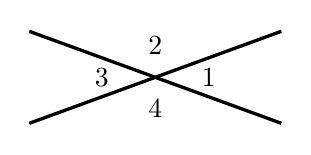
\begin{tikzpicture}[scale=0.8]\draw[very thick] (-2,-0.73)--(2,0.73); \draw[very thick] (-2,0.73)--(2,-0.73); \node at (0.85,0){$1$}; \node at (0,0.5){$2$}; \node at (-0.85,0){$3$}; \node at (0,-0.5){$4$};\end{tikzpicture}\end{minipage}\hfill
\begin{minipage}[c]{0.67\linewidth}\renewcommand{\arraystretch}{1.7}\begin{tabular}{@{}l l@{}}
$m\angle 1 + m\angle 2 = 180^\circ$ & \fb[4cm]{Linear Pair Postulate}\\
$m\angle 3 + m\angle 2 = 180^\circ$ & \fb[4cm]{Linear Pair Postulate}\\
$\angle 1 \cong \angle 3$ & \fb[5.2cm]{Congruent Supplements Theorem}\\
\end{tabular}\end{minipage}\end{watchme}

\vid{Use it to find angles}
\begin{watchme}Same picture: $m\angle 1 = 3x + 10$, \ $m\angle 3 = 5x - 30$.\par\vspace{1mm}
\renewcommand{\arraystretch}{1.7}\begin{tabular}{@{}l l@{}}
$3x + 10 = 5x - 30$ & vertical angles are \fb[2.2cm]{congruent}\\
$40 = 2x$, \ $x = $ \fb[1.2cm]{$20$} & solve\\
$m\angle 1 = 3(20) + 10 = $ \fb[1.4cm]{$70^\circ$} & \\
$m\angle 2 = 180 - 70 = $ \fb[1.4cm]{$110^\circ$} & $\angle 1$ and $\angle 2$ are a \fb[2.2cm]{linear pair}\\
\end{tabular}\end{watchme}

\vid{Watch out}
\begin{mistakebox}Vertical angles are \fb[1.6cm]{across} from each other --- they are equal. Angles \fb[1.6cm]{next to} each other on a line are a linear pair --- they add to $180^\circ$, they are \fb[1cm]{not} equal.\end{mistakebox}

\vid{Your turn}
\begin{yourturn}$\angle A$ and $\angle B$ are both supplementary to $\angle C$. \quad $m\angle A = 2x + 15$, \ $m\angle B = 3x - 5$. \ Find $x$ and $m\angle A$.\par\vspace{2mm}
Congruent \fb[2.6cm]{Supplements}: \ $2x + 15 = 3x - 5$ \ $\Rightarrow$ \ $x = $ \fb[1.2cm]{$20$}, \quad $m\angle A = $ \fb[1.4cm]{$55^\circ$}\end{yourturn}

\begin{notebox}\textbf{Remember:}\quad Linear pair: adds to $180^\circ$.\quad Vertical angles: congruent.\quad All right angles are congruent.\quad Supplementary (or complementary) to the \textbf{same} angle $\Rightarrow$ congruent.\end{notebox}
\end{document}
